

\documentclass{beamer}
 
\usepackage[utf8]{inputenc}
\usepackage{listings}

\usepackage{listings}
\usepackage{color}
\usepackage{enumitem}
\usepackage{hyperref}


\definecolor{dkgreen}{rgb}{0,0.6,0}
\definecolor{gray}{rgb}{0.5,0.5,0.5}
\definecolor{mauve}{rgb}{0.58,0,0.82}

\lstset{frame=tb,
  language=C++,
  aboveskip=3mm,
  belowskip=3mm,
  showstringspaces=false,
  columns=flexible,
  basicstyle={\small\ttfamily},
  numbers=left,
  numberstyle=\tiny\color{gray},
  keywordstyle=\color{blue},
  morekeywords={vector},
  commentstyle=\color{dkgreen},
  stringstyle=\color{mauve},
  breaklines=true,
  breakatwhitespace=true,
  tabsize=3
}



\definecolor{lmugreen}{RGB}{50,55,44}
 
\setbeamercolor{title}{fg=lmugreen}
\setbeamercolor{titlelike}{fg=lmugreen}
%\setbeamertemplate{itemize items}[circle]
\setbeamertemplate{itemize items}{\color{black}$\blacktriangleright$}
%\setbeamertemplate{footline}[frame number]

\setbeamertemplate{footline}[text line]{%
  \parbox{\linewidth}{\vspace*{-8pt}c3particles\hfill\insertshortauthor\hfill\insertframenumber/\inserttotalframenumber}}
\setbeamertemplate{navigation symbols}{}

 
%Information to be included in the title page:
\title{c3particles \\ Modellierung eines Partikelsystems in C++}
\subtitle{Praktikumsabschlusspr\"asentation}
\author{Rosalie Kletzander}
\institute{Institut f\"ur Informatik, LMU M\"unchen}
\date{6.8.2017}
 
\usebackgroundtemplate%
{%
    
\includegraphics[width=\paperwidth,height=\paperheight]{images/bg-empty.pdf}%
}
\setbeamertemplate{frametitle}[default][center]
 
\begin{document}
 
\frame{\titlepage}
 
\begin{frame}
\frametitle{Zielsetzung}
- Partikelsystem: Simulation (oft in der 3d Grafik) von chaotischen Systemen und nat\"urlichen Ph\"anomenen \linebreak
\linebreak
- C++ als Werkzeug: mathematisch Ausdrucksstark, formale Konzepte lassen sich sauber definieren \linebreak
\linebreak
- Ziel: Entwicklung einer Programmierabstraktion f\"ur Newton'sche Mechanik in Parntikelsystemen

\end{frame}

\begin{frame}
\frametitle{Newton'sche Gesetze}
\begin{itemize}[label={}]
 \item<1-> "Ein Körper verharrt im Zustand der Ruhe [..] sofern er nicht durch einwirkende Kr\"afte zur \"Anderung seines Zustands gezwungen wird."
 \item
 \item<2-> "Das Verh\"altnis zwischen der Masse eines Objekts, seiner Beschleunigung und der angewandten Kraft ist F = m*a"
 \item
 \item<3-> $\rightarrow$ brauchen \emph{Kr\"afte}, um Beschleunigungen zu erreichen
\end{itemize}
\end{frame}

\begin{frame}
\frametitle{Physikalische Grundlagen}
\begin{itemize}[label={}]
 \item<1-> \begin{equation}
a = F/m
\end{equation}
\item<2->
\begin{equation}
\overrightarrow{v}(t) = \int \mathrm{(\overrightarrow{a})} \mathrm{d}t = \overrightarrow{a}*t + C_v
\end{equation}
 \item<3-> \begin{align}
\overrightarrow{s}(t) = \int \mathrm{(\overrightarrow{v})} \mathrm{d}t = \int (\overrightarrow{a}*t + C_v) \mathrm{d}t \\ = \frac{\overrightarrow{a}*t^2}{2} + C_v + C_s
\end{align}
\end{itemize}
\end{frame}


\begin{frame}
\frametitle{Physikalische Grundlagen}
Das Superpositionsprinzip: \linebreak
\linebreak
"Wirken auf ein Objekt mehrere Kräfte, so addieren sich diese vektoriell zu einer resultierenden Kraft auf."
\linebreak
\begin{equation}
\overrightarrow{F_{res}} = \overrightarrow{F_1} + \overrightarrow{F_2} +...+ \overrightarrow{F_n}
\end{equation}
\end{frame}

\begin{frame}
\frametitle{Modellierung}
- Modellierung des Partikelsystems basiert stark auf der Physik \linebreak
\linebreak
- besteht aus Newton'schen Objekten (Partikeln) und Kr\"aften \linebreak
$\rightarrow$ Konzepte \linebreak
\linebreak
- die Expressions m\"ussen die Gesetze der Physik erf\"ullen k\"onnen
\end{frame}


\begin{frame}
\frametitle{Modellierung}

Expressions f\"ur "Newton'sches Objekt" \linebreak
\linebreak
- $F=m*a \rightarrow$  "apply\_force(NO)", oder "$NO << Kraft$" \linebreak
\linebreak
- Berechnung der Position $\rightarrow$ "update(NO)"
\end{frame}

\begin{frame}
\frametitle{Modellierung}

Expressions f\"ur "Kraft" \linebreak
\linebreak
- Ausl\"oser f\"ur eine Kraft $\rightarrow$ "calc\_force(NO, NO, ff)" \linebreak
\linebreak
- Superpositionsprinzip $\rightarrow$ "accumulate(f1, f2, ..)"
\end{frame}

\begin{frame}
\frametitle{Implementierung}
\textbf{
\begin{figure}[]
\centering
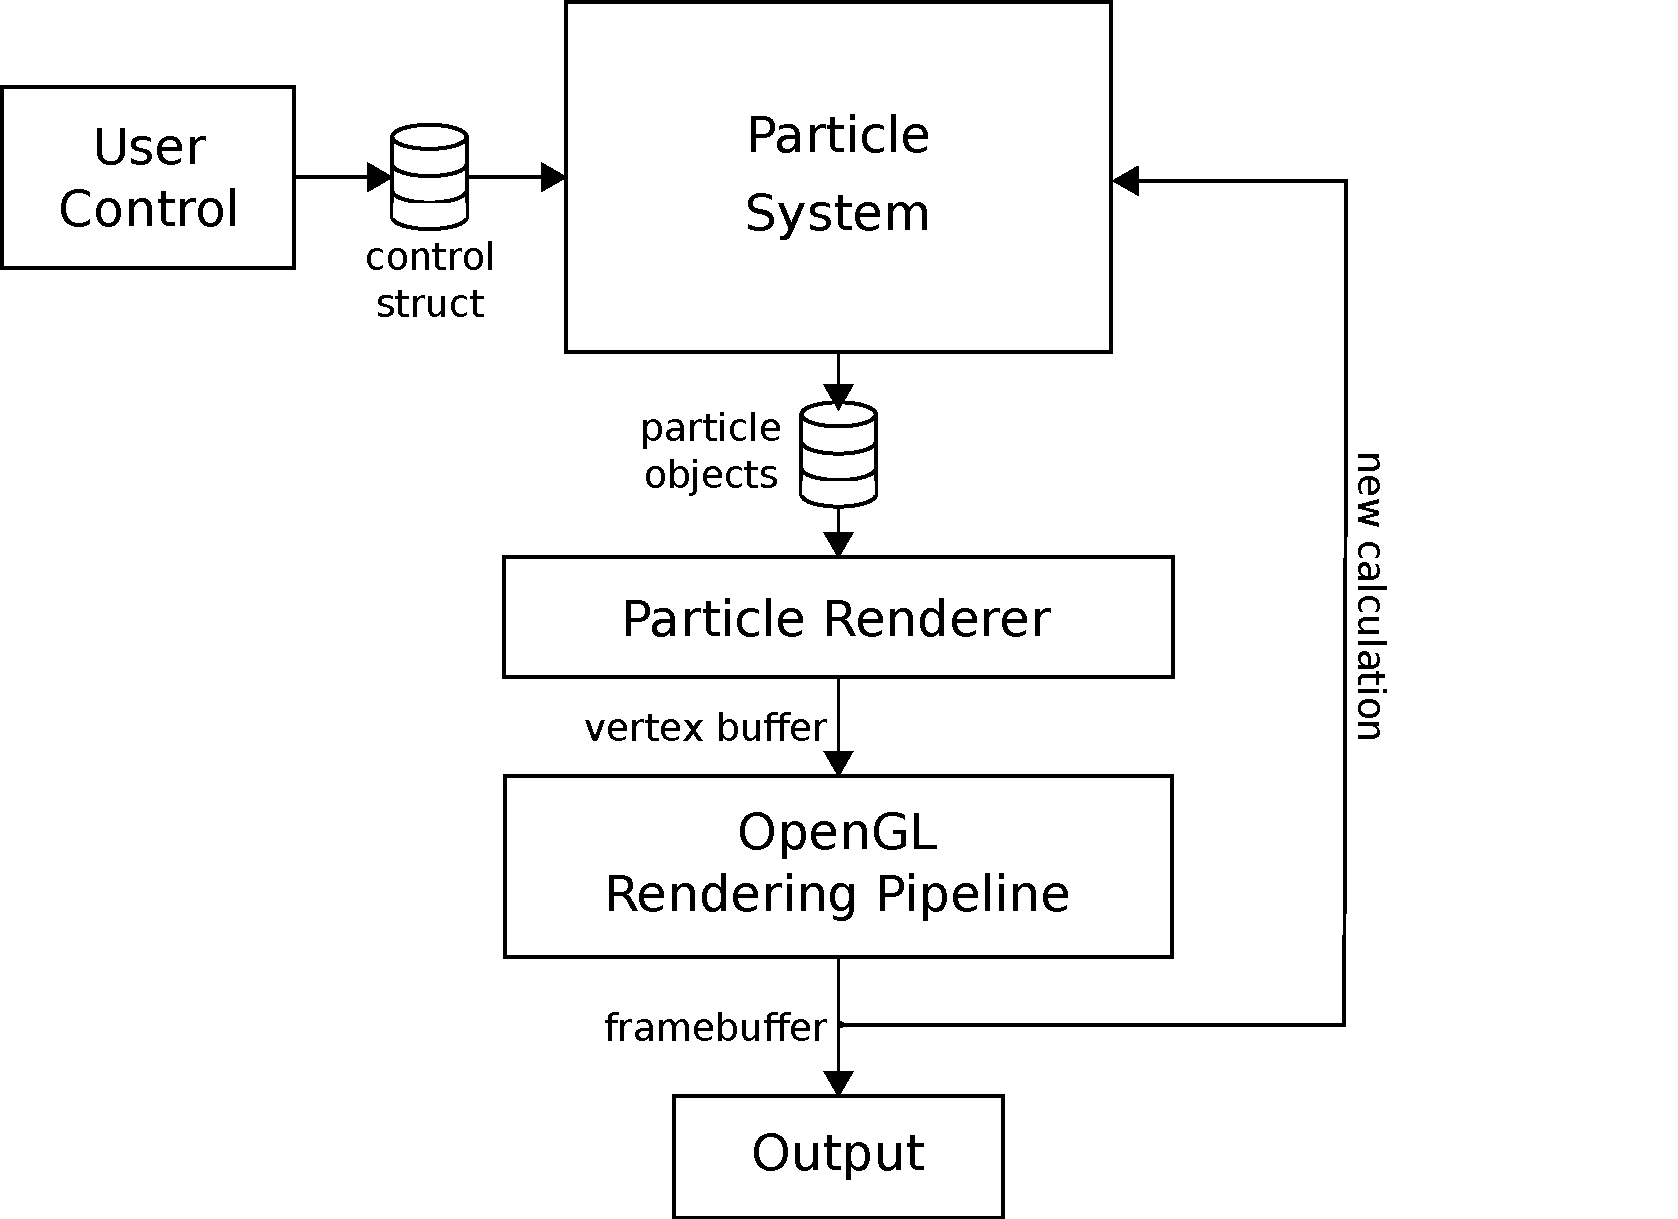
\includegraphics[width=0.8\textwidth]{../images/system-diagram-no-shaders.pdf}
\caption{Systemdiagramm}
\label{fig:sysdia}
\end{figure}
}
\end{frame}

\begin{frame}
\frametitle{Implementierung}
\begin{figure}[]
\centering
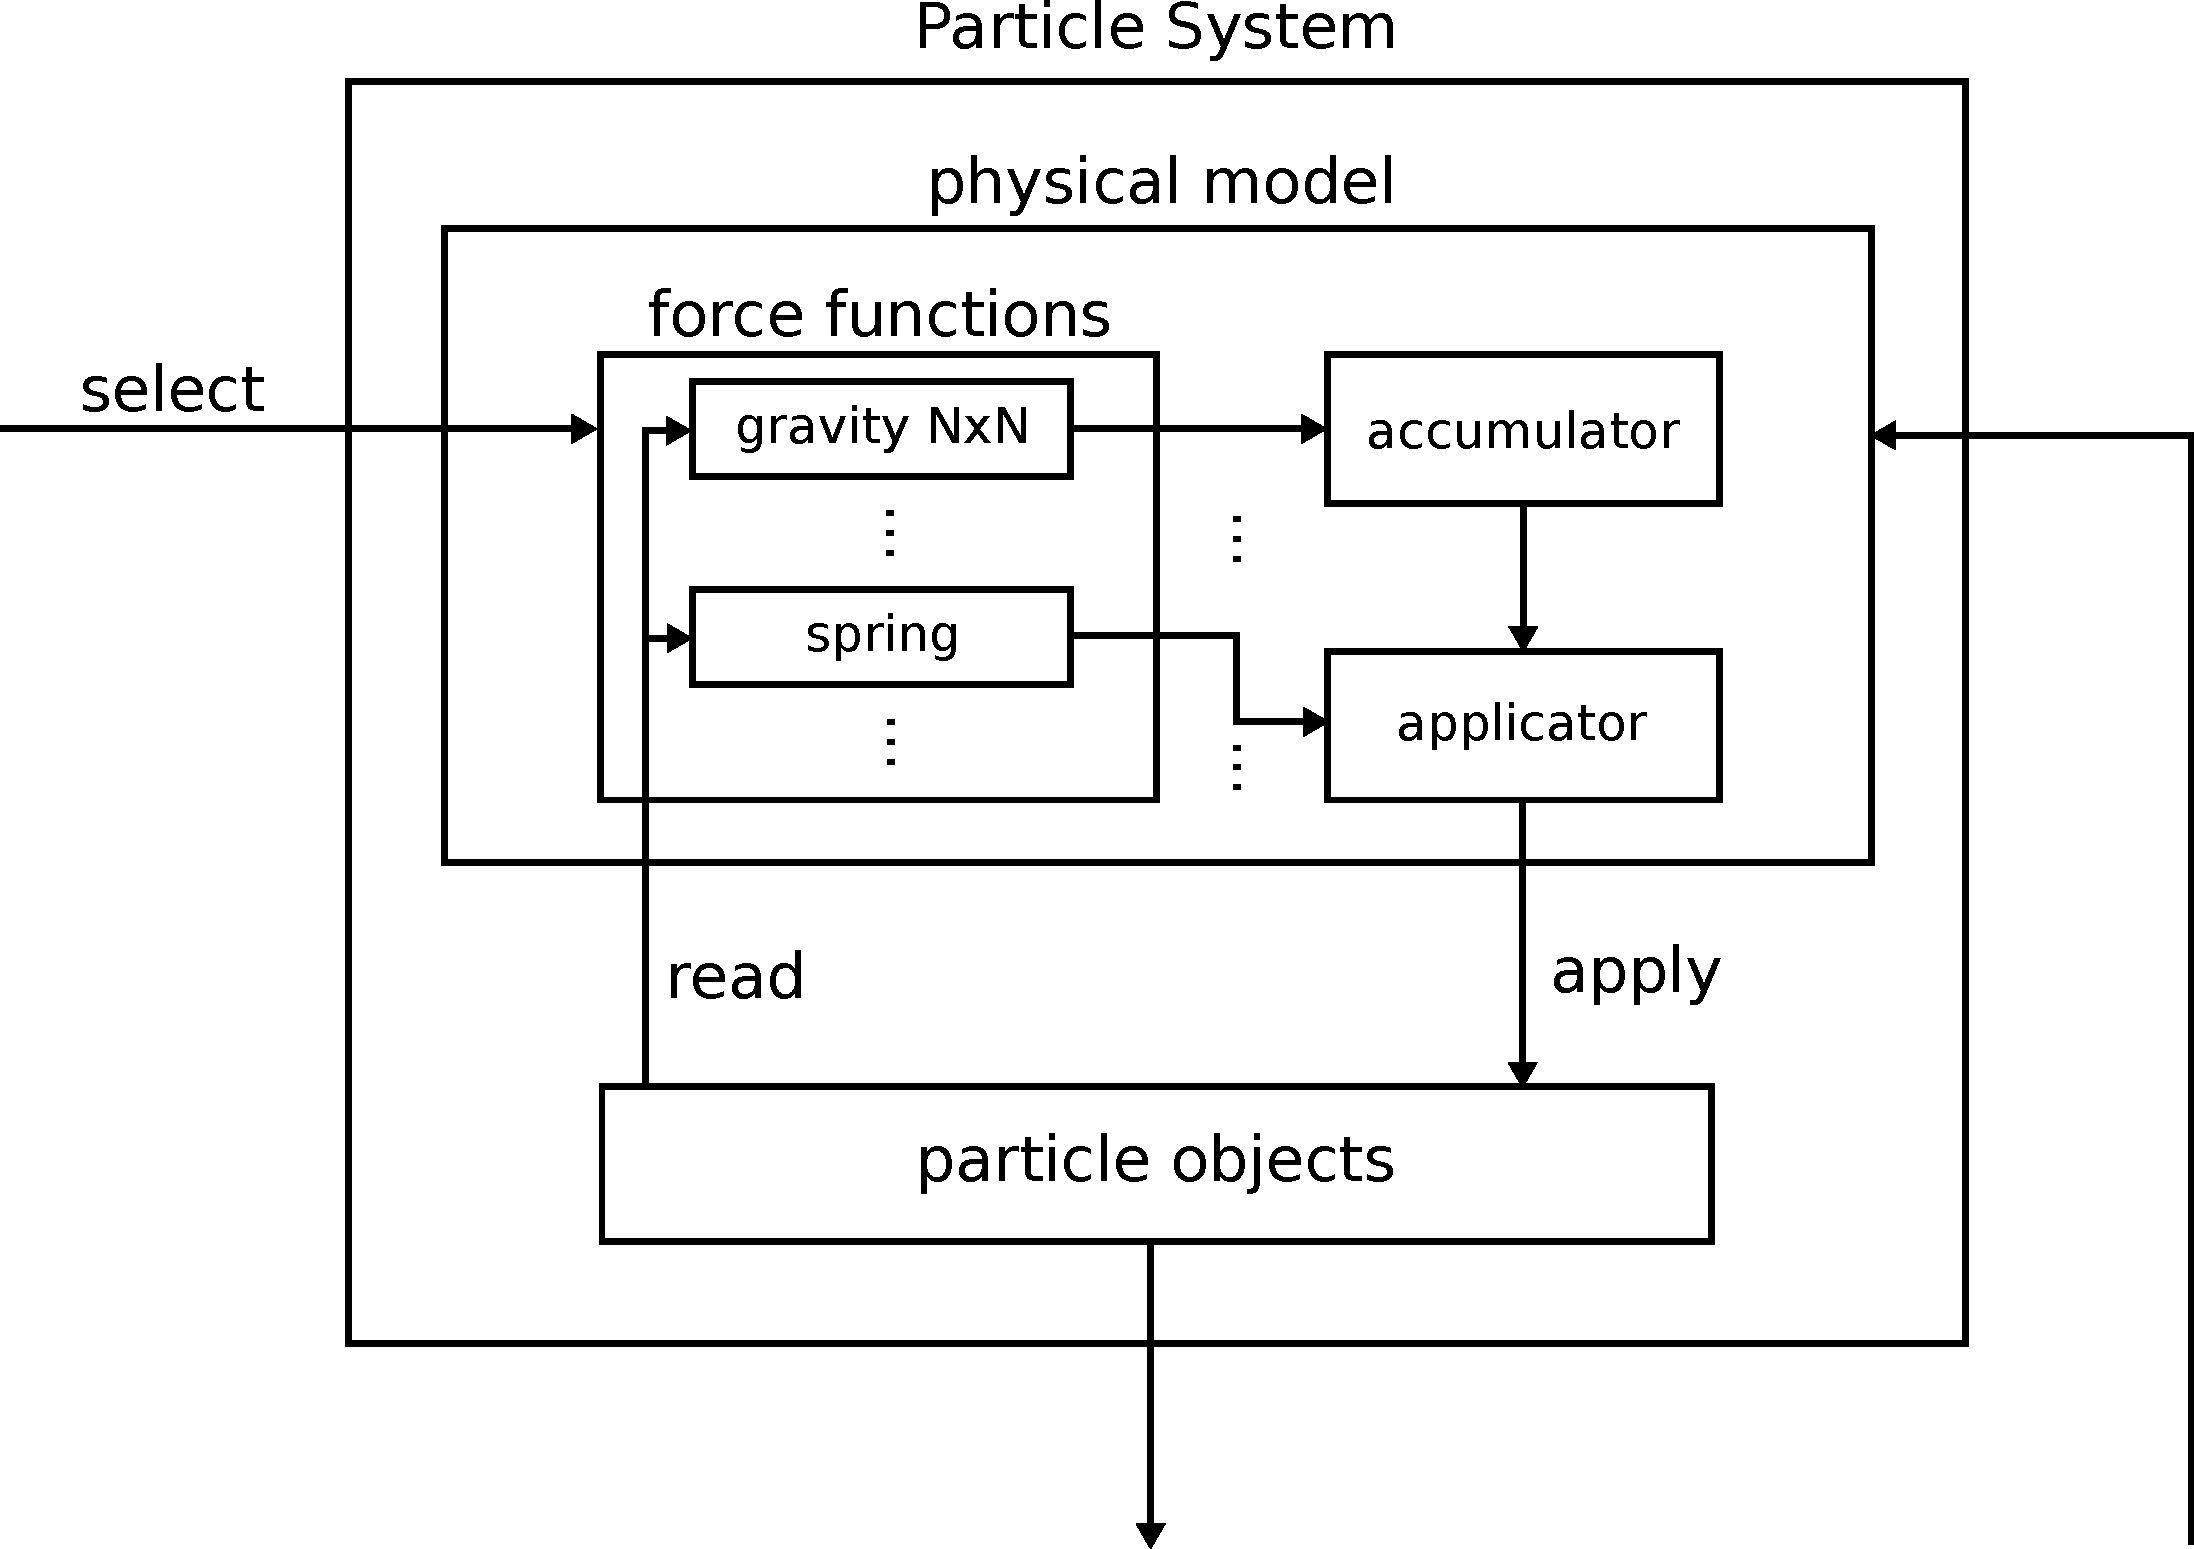
\includegraphics[width=0.8\textwidth]{../images/particle-system-detail.pdf}
\caption{Das Partikelsystemmmodell im Detail}
\label{fig:sysdiadetail}
\end{figure}
\end{frame}

\begin{frame}
\frametitle{Implementierung}
\begin{figure}[]
\centering
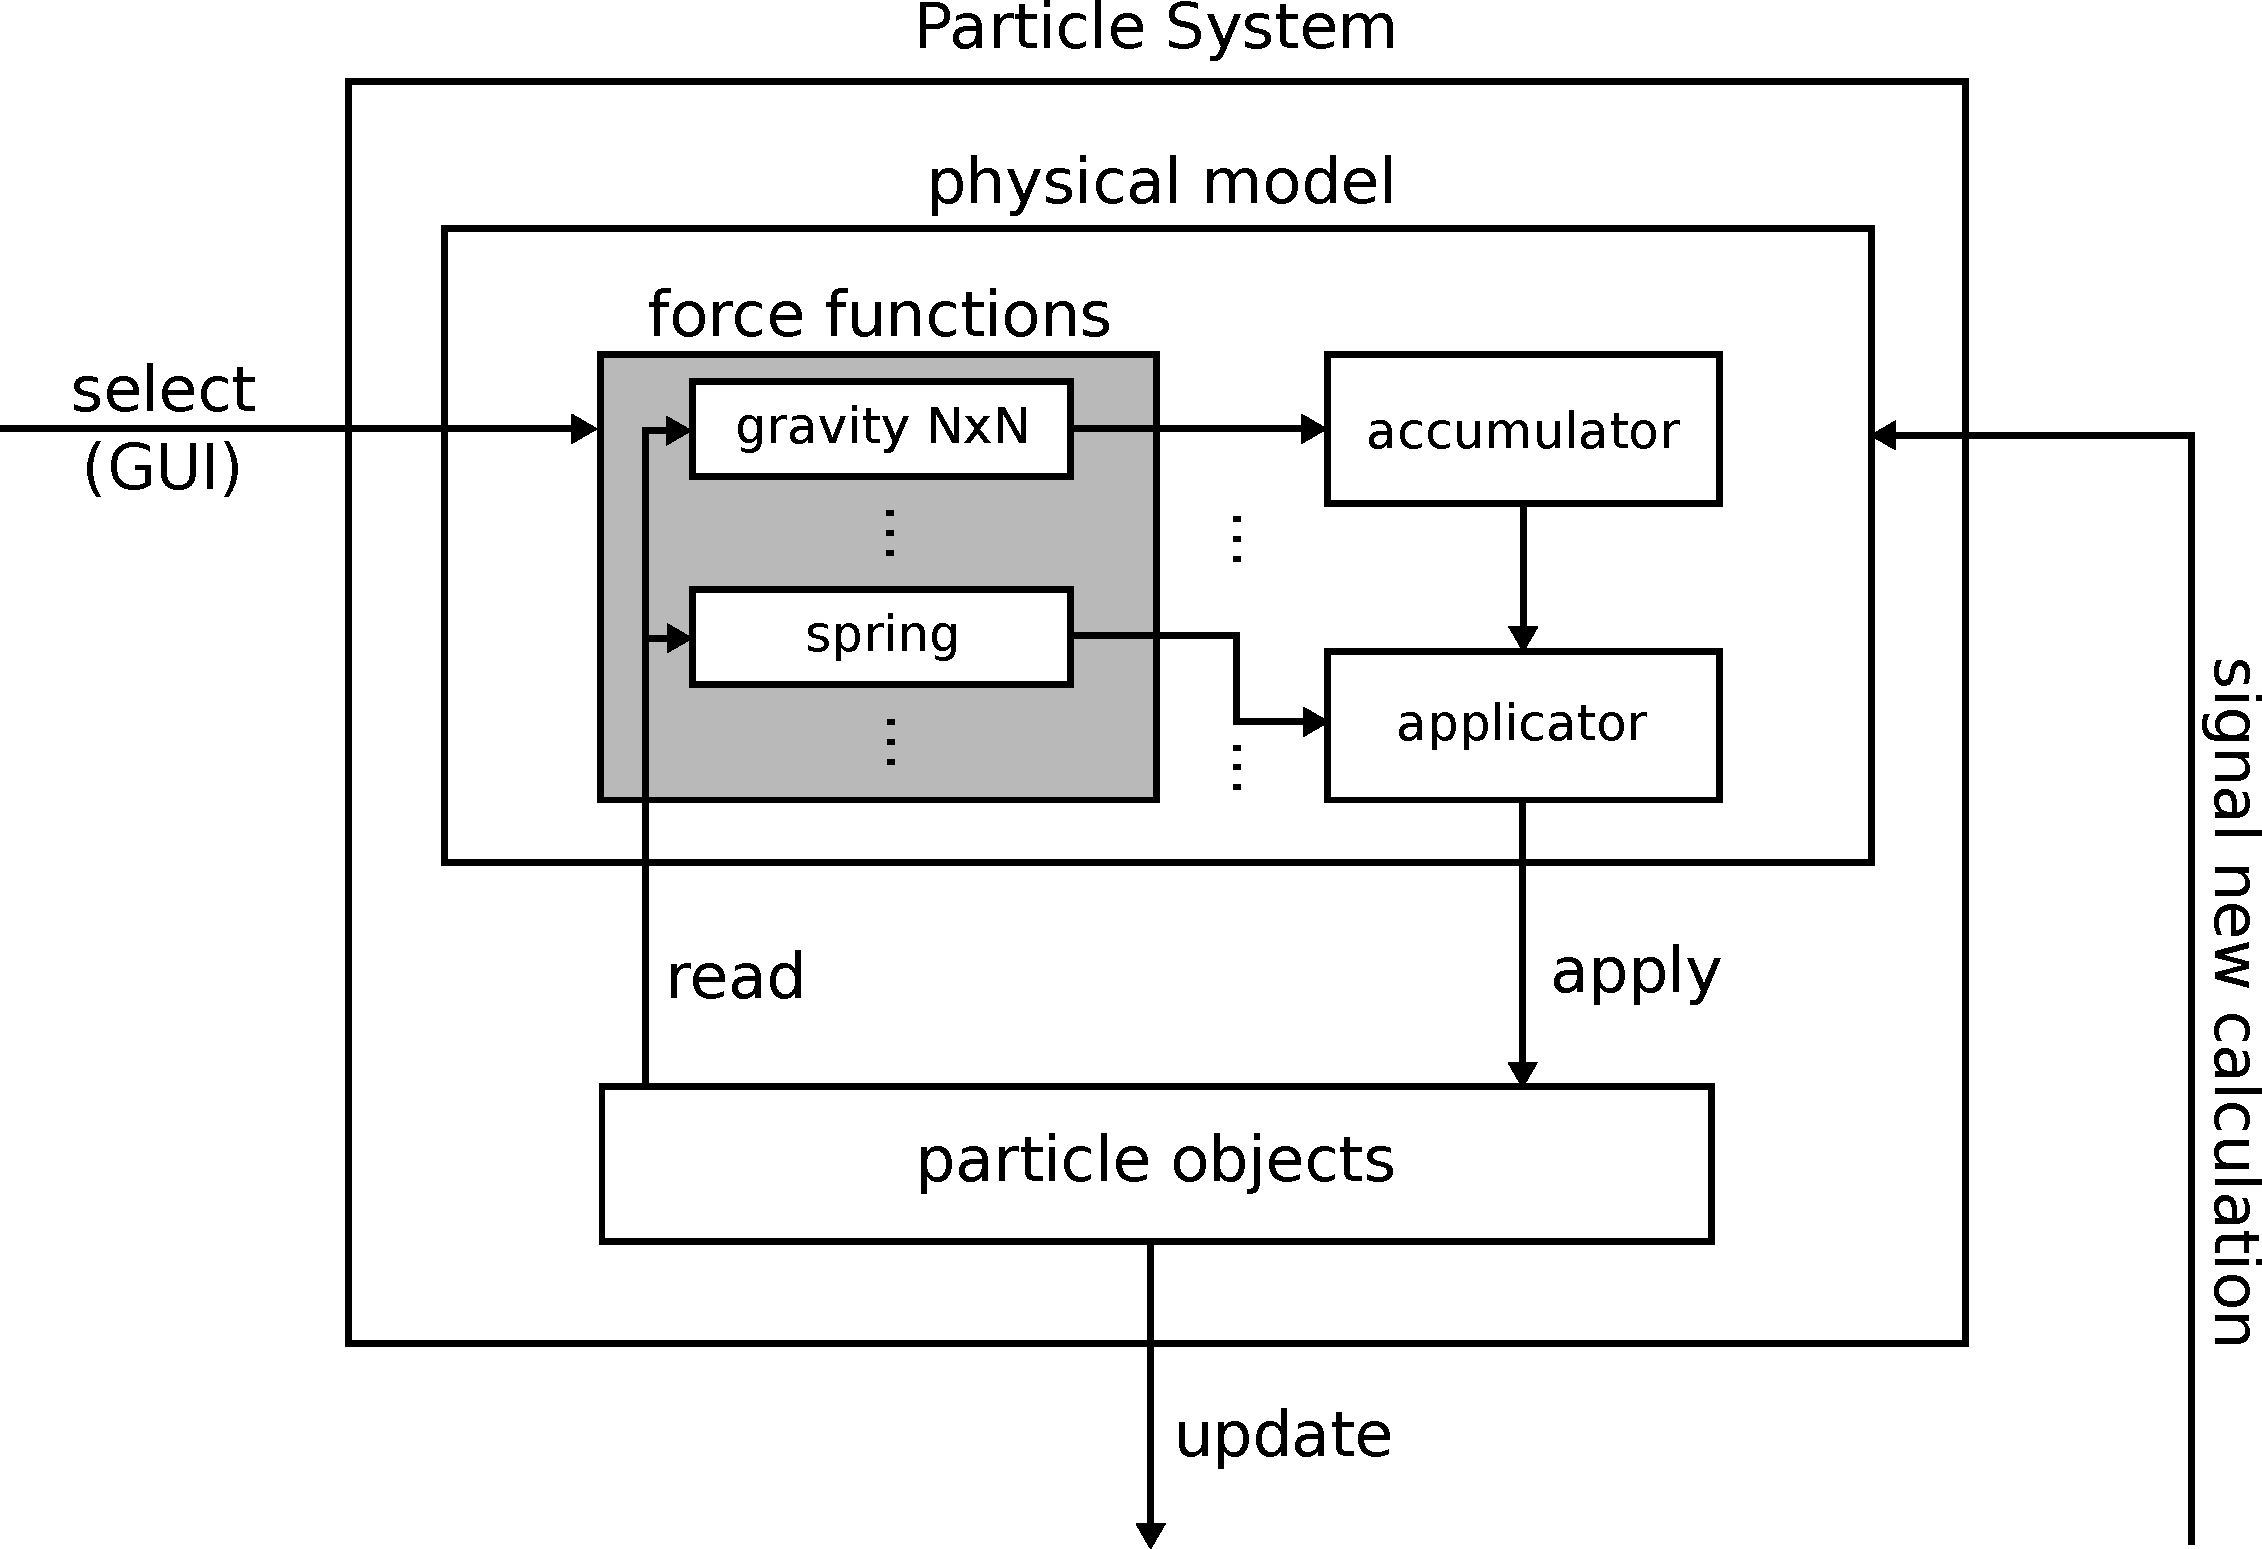
\includegraphics[width=0.8\textwidth]{images/detail1.pdf}
\caption{Die Kraftfunktionen (basierend auf calc\_force)}
\end{figure}
\end{frame}

%\begin{frame}[fragile]
%\frametitle{Implementierung}
%\begin{lstlisting}[caption=gravity function]
%// uses calc_force to calculate gravitational force between two particles
%Force gravity(const Particle &p1, const Particle &p2, float g_constant)
%{
%  Force result = calc_force(p1, p2, 
%						[p1, p2](const Particle &, const Particle &) {
%	glm::vec3 direction = p2.location - p1.location;
%	float gforce = (p1.mass * p2.mass) / pow(glm::length(direction), 2);
%	glm::normalize(direction);
%
%	return g_constant * (gforce * direction);
%  });
%}               
%\end{lstlisting}
%\end{frame}

\begin{frame}
\frametitle{Implementierung}
\begin{figure}[]
\centering
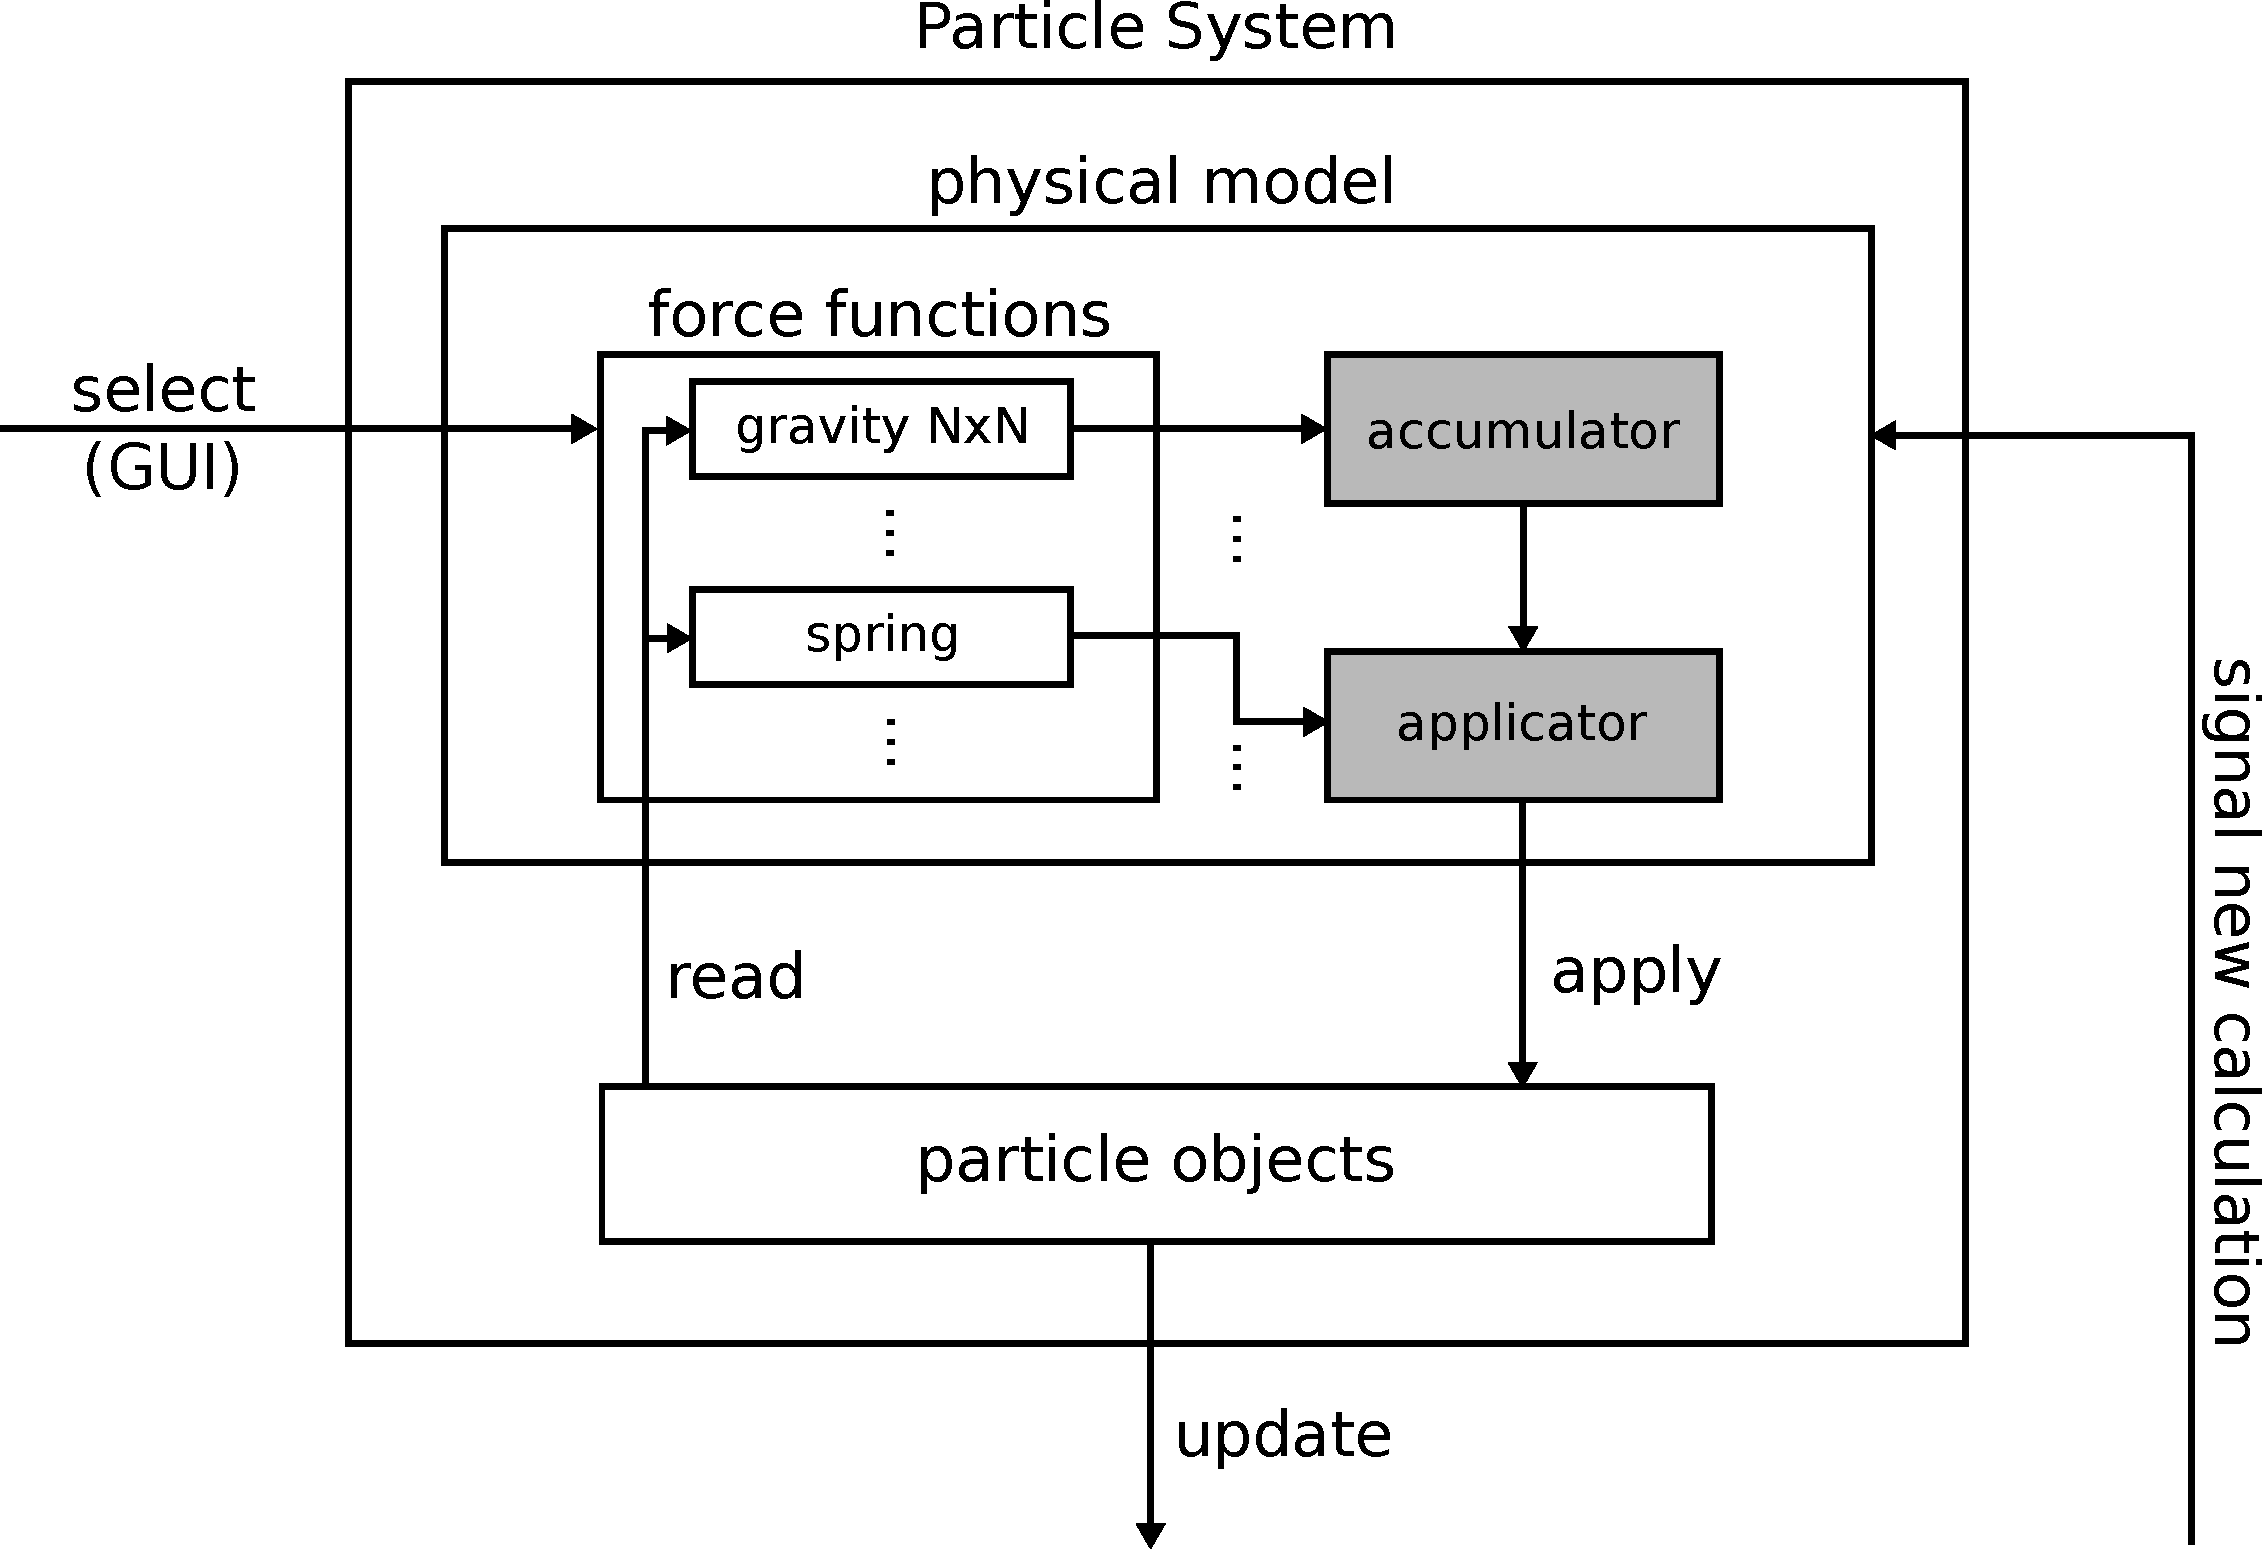
\includegraphics[width=0.8\textwidth]{images/detail2.pdf}
\caption{Externe vs Inter-Partikel Kr\"afte}
\end{figure}
\end{frame}

%\begin{frame}
%NxN
%\end{frame}

\begin{frame}[fragile]
\frametitle{Implementierung}
\begin{lstlisting}[caption=Beispiel von Berechnung und Anwendung von Kr\"aften]
//iterate over all particles in the particle system
std::for_each(ps.begin(), ps.end(), [&ps](c3p::Particle& p)
{
	// simple user-defined attraction force
	p << calc_force(p, Particle(), [p](const Particle &, const Particle &)
	{
    	glm::vec3 direction = glm::normalize(glm::vec3(0,0,0) - p.location());
		return direction * 0.1;
    });
    
    // spring force from virtual particle at (0,0,0) to each particle
	p << spring(p, Particle(0,0,0), {spring_constant, spring_length);
   					 
	...
\end{lstlisting}
\end{frame}

\begin{frame}[fragile]
\frametitle{Implementierung}
\begin{lstlisting}[caption=Beispiel von Berechnung und Anwendung von Kr\"aften]
	...

    //gravitational forces between particles
	p << c3p::accumulate(p,
						 ps.particles(),
						 {ps.g_constant()},
    					 c3p::gravity);
}          
   
\end{lstlisting}
\end{frame}

\begin{frame}
\frametitle{Implementierung}
\begin{figure}[]
\centering
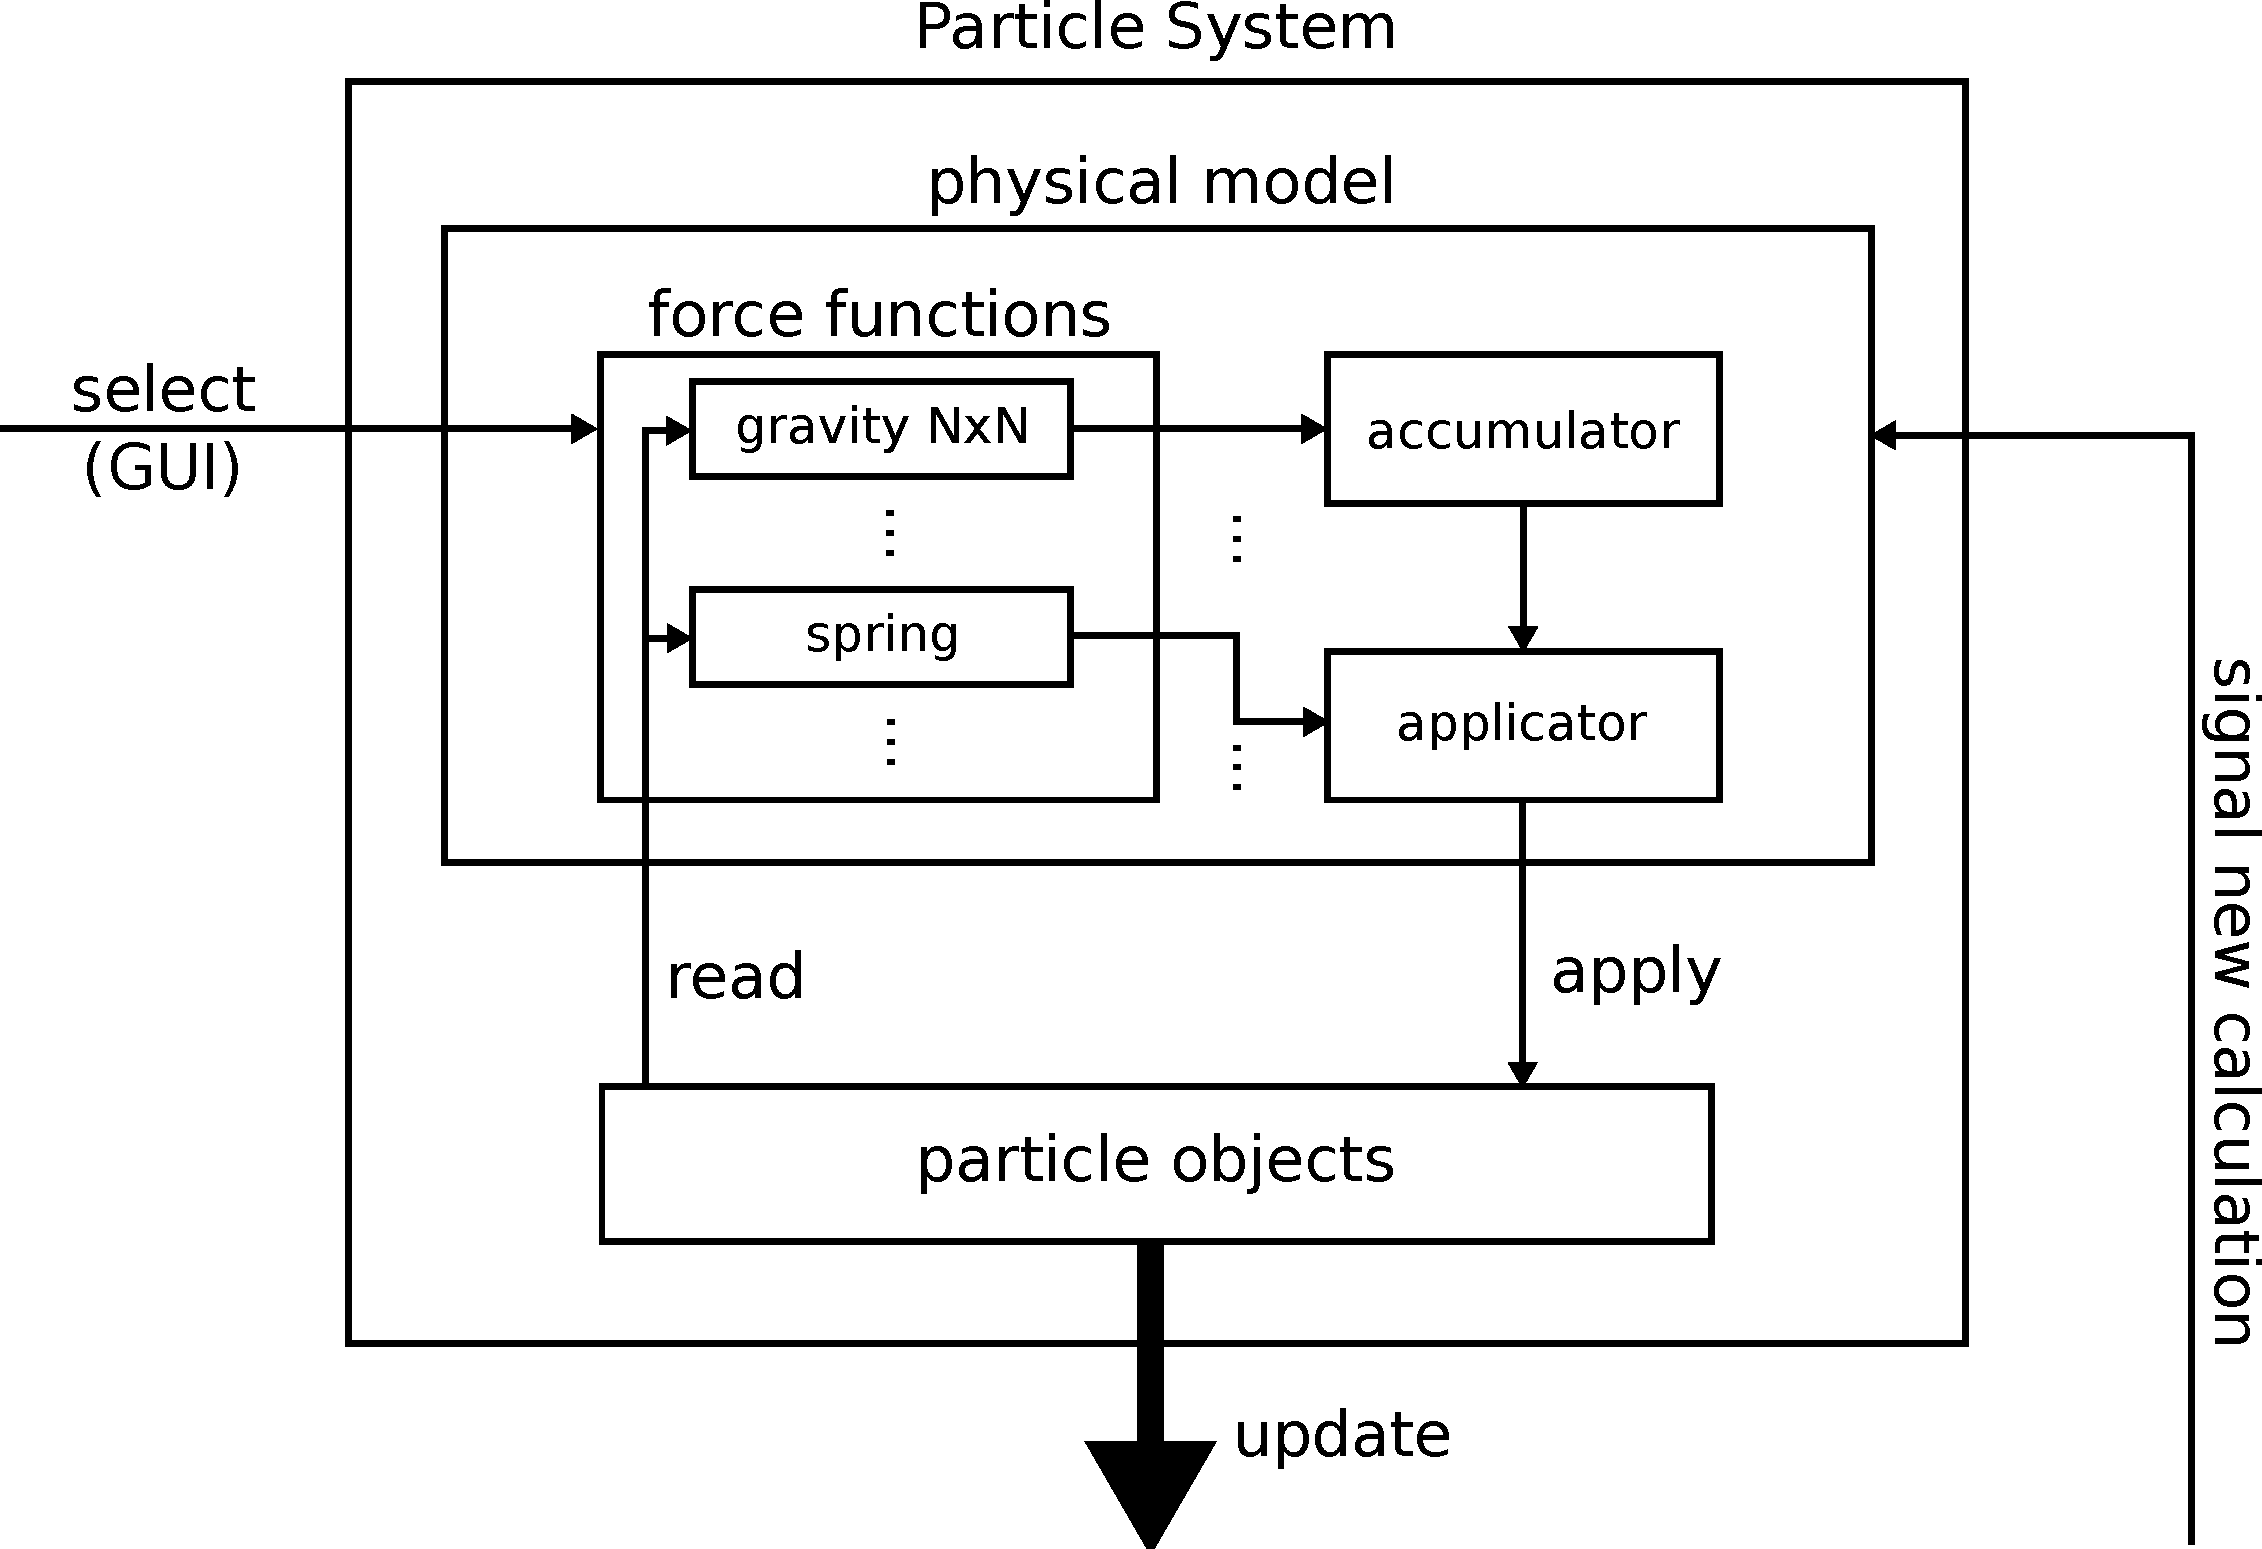
\includegraphics[width=0.8\textwidth]{images/detail3.pdf}
\caption{Aktualisieren der Geschwindigkeit und des Orts}
\end{figure}
\end{frame}


\begin{frame}[fragile]
\frametitle{Implementierung}
\begin{lstlisting}[caption=Update Funktion]
void update(Particle &p)
{
	//v(t) = a*t + v(t-1)                                                            
	p.velocity = p.acceleration * 1.0f + p.velocity; //deltaT = 1.0                                  
                                                                                           
	//s(t) = (a*t^2)/2 + v(t) + s(t-1)                                               
	p.location = (p.acceleration * 1.0f) / 2.0f + p.velocity + p.location;
                                       	
	//acceleration is not accumulative, but recalculated at each time step          
	p.acceleration = {0, 0, 0};
}                                                            
\end{lstlisting}
\end{frame}

\begin{frame}
\frametitle{M\"ogliche Optimierungen}
\begin{itemize}[label={}]
 \item<1->- Parallelisierung der Iterationsschleifen \"uber die Partikel
 \item
 \item<2->- Offloading auf die GPU
 \item
 \item<3->- Partitionierte, semi-symmetrische Kr\"aftematrix
\end{itemize}
\end{frame}


\begin{frame}
\frametitle{Zusammenfassung}
\begin{columns}[T] % align columns
\begin{column}{.33\textwidth}
%\color{black}\rule{\linewidth}{4pt}
Physik $\rightarrow$ \linebreak
\linebreak
\linebreak

\tiny$\overrightarrow{s}(t) = \frac{\overrightarrow{a}*t^2}{2} + C_v + C_s$
\linebreak
\linebreak
\linebreak
\linebreak
\tiny$F= m*a$
\linebreak
\linebreak
\linebreak
\linebreak
\tiny$\overrightarrow{F_{res}} = \overrightarrow{F_1} + \overrightarrow{F_2} +... \overrightarrow{F_n}$

\end{column}%
\hfill%
\begin{column}{.33\textwidth}
%\color{black}\rule{\linewidth}{4pt}

Konzepte $\rightarrow$ \linebreak
\linebreak

\tiny"Newton'sches Objekt" \linebreak
\linebreak
"$NO << Kraft$" \linebreak
\linebreak
"update(NO)"\linebreak
\linebreak
\linebreak

"Kraft" \linebreak
\linebreak
"calc\_force(NO, NO, ff)" \linebreak
\linebreak
"accumulate(f1, f2, ..)"
\end{column}%
\begin{column}{.33\textwidth}
%\color{black}\rule{\linewidth}{4pt}

Implementierung\linebreak
\linebreak
\begin{figure}[]
\centering
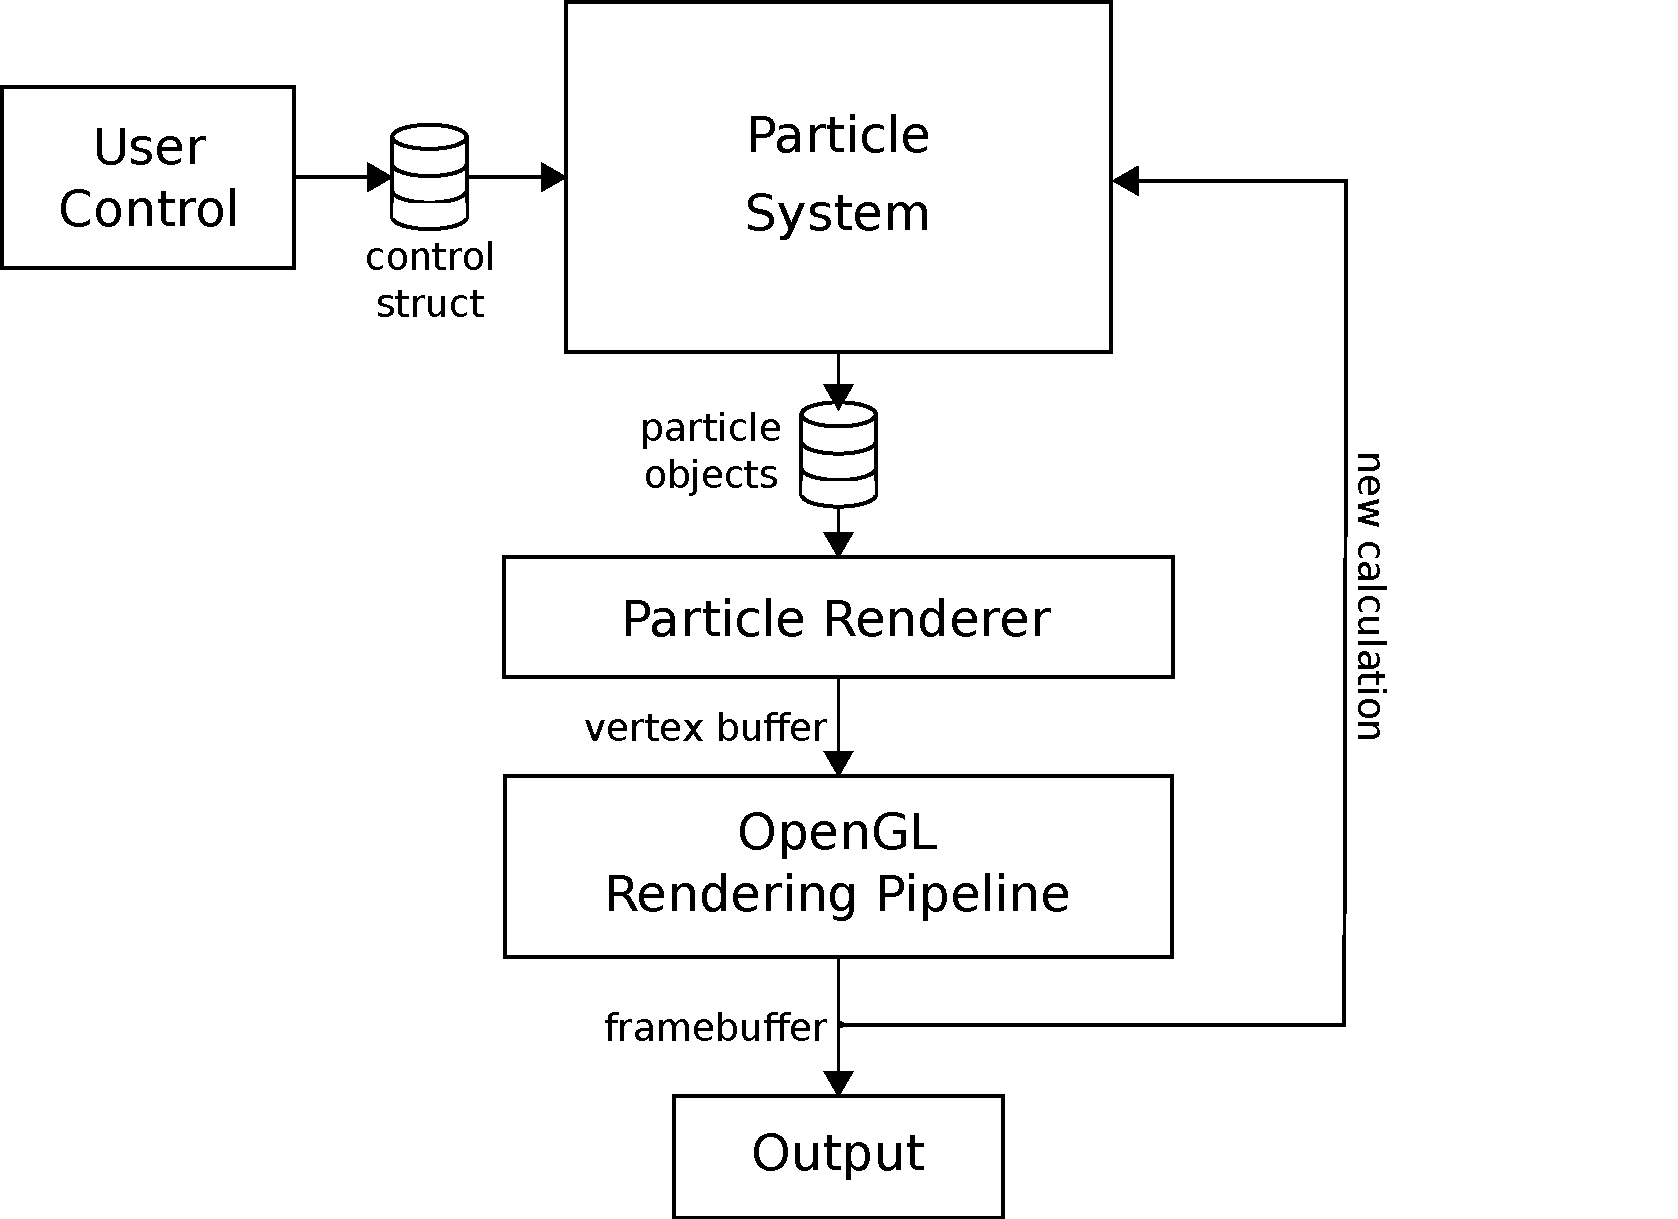
\includegraphics[width=\textwidth]{../images/system-diagram-no-shaders.pdf}
\end{figure}

\end{column}%
\end{columns}
\end{frame}


\end{document}

